%Background image credits:https://commons.wikimedia.org/wiki/File:CannabisBud.jpg Thomas Elliott, CC0, via Wikimedia Commons
\documentclass[a4paper, 11pt, oneside, polutonikogreek, english]{article}
\usepackage{lmodern}
\usepackage[T1]{fontenc}
% Load encoding definitions (after font package)
\usepackage[dvipsnames]{xcolor}
\usepackage{eso-pic,graphicx}
\usepackage[top=57mm, bottom=57mm, outer=33mm, inner=33mm]{geometry}
\setlength{\columnsep}{90pt}
\definecolor{customPurple}{RGB}{221,229,194}
% Load encoding definitions (after font package)

% Load encoding definitions (after font package)

\usepackage{textalpha}

\usepackage{listings}
\lstset{basicstyle=\ttfamily}
\usepackage{pdflscape}

% Babel package:
\usepackage[english]{babel}
\usepackage{wasysym}

% With XeTeX$\$LuaTeX, load fontspec after babel to use Unicode
% fonts for Latin script and LGR for Greek:
\ifdefined\luatexversion \usepackage{fontspec}\fi
\ifdefined\XeTeXrevision \usepackage{fontspec}\fi

% ``Lipsiakos'' italic font `cbleipzig`:
\newcommand*{\lishape}{\fontencoding{LGR}\fontfamily{cmr}%
		       \fontshape{li}\selectfont}
\DeclareTextFontCommand{\textli}{\lishape}

\usepackage{booktabs}
\usepackage{graphicx}
\setlength{\emergencystretch}{15pt}
\graphicspath{ {./ } }
\usepackage[figurename=]{caption}
\usepackage{float}
\usepackage{fancyhdr}
\usepackage{microtype}

\usepackage{setspace}
\onehalfspacing

% change color of text, example replace all \color{Goldenrod} with \color{lightgray}

\makeatletter % change only the display of \thepage, but not \thepage itself:
\patchcmd{\ps@plain}{\thepage}{\color{customPurple}{\thepage}}{}{}
\makeatother

\color{customPurple}

\begin{document}
\bfseries
\AddToShipoutPictureBG{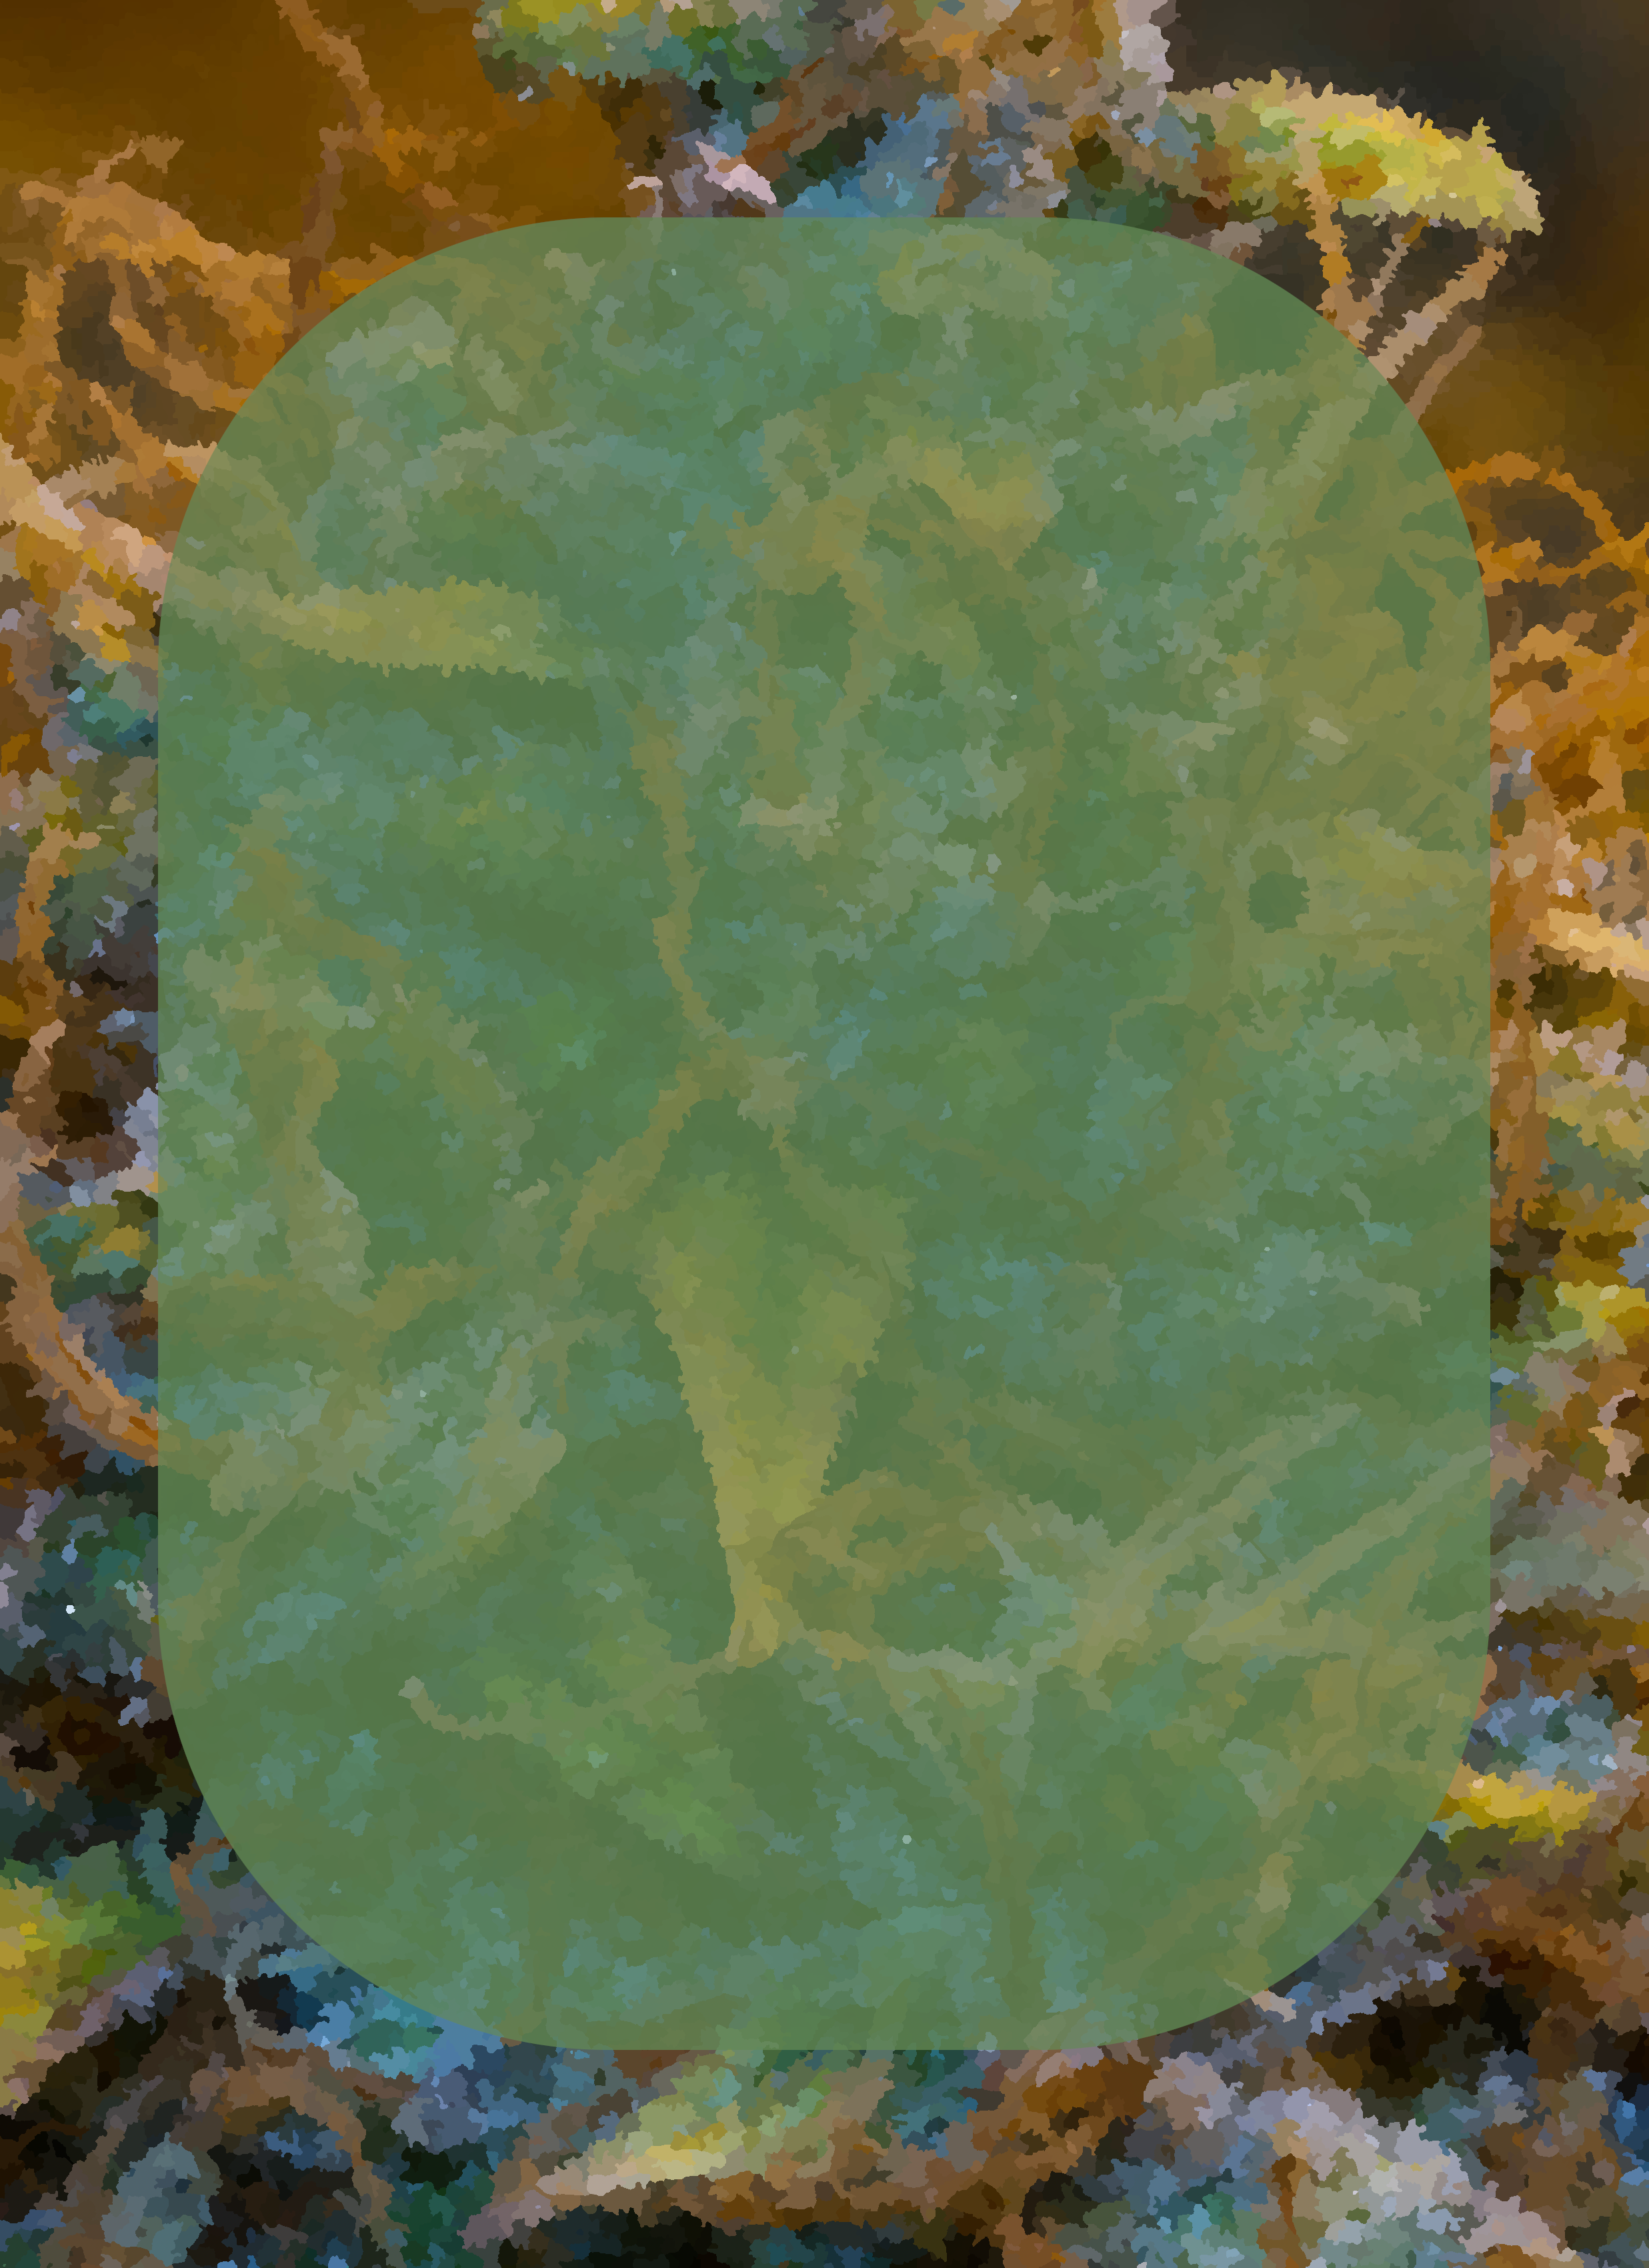
\includegraphics[width=\paperwidth,height=\paperheight]{CannabisBud.png}}
\begin{titlepage} % Suppresses headers and footers on the title page
	\centering % Centre everything on the title page
	\scshape % Use small caps for all text on the title page

	%------------------------------------------------
	%	Title
	%------------------------------------------------
	
	\rule{\textwidth}{1.6pt}\vspace*{-\baselineskip}\vspace*{2pt} % Thick horizontal rule
	\rule{\textwidth}{0.4pt} % Thin horizontal rule
	
	\vspace{0.75\baselineskip} % Whitespace above the title

        {\LARGE On the Preparations of the Indian Hemp,\\ or Gunjah,\\ (\emph{Cannabis Indica})} % Title
	
	\vspace{0.75\baselineskip} % Whitespace below the title
	
	\rule{\textwidth}{0.4pt}\vspace*{-\baselineskip}\vspace{3.2pt} % Thin horizontal rule
	\rule{\textwidth}{1.6pt} % Thick horizontal rule
	
	\vspace{1\baselineskip} % Whitespace after the title block
	
	%------------------------------------------------
	%	Subtitle
	%------------------------------------------------
	
	{Their Effects on the Animal System in Health, and their Utility in the Treatment of Tetanus and other convulsive Disorders.} % Subtitle or further description
	
	\vspace*{1\baselineskip} % Whitespace under the subtitle
	
	%------------------------------------------------
	%	Editor(s)
	%------------------------------------------------
	
	\vspace{1\baselineskip} % Whitespace before the editors

        {By \Large William Brooke O'Shaughnessy, MD,\\\small Assistant Surgeon; Professor of Chemistry, Medical College, Kolkata; --- and officiating Joint-Secretary to the Asiatic Society of Bengal.}

    %------------------------------------------------
	%	Cover photo
	%------------------------------------------------
	
	%\includegraphics[scale=1]{cover}
	
	%------------------------------------------------
	%	Publisher
	%------------------------------------------------
		
	\vspace*{\fill}% Whitespace under the publisher logo
	
	% Publication year
	
	{Kolkata, 1839} % Publisher
 
        {\small Bishop's College Press}

	\vspace{1\baselineskip} % Whitespace under the publisher logo

        Internet Archive Online Edition  % Publication year
	
	{\small Attribution NonCommercial ShareAlike 4.0 International } % Publisher
\end{titlepage}
\clearpage
\setlength{\parskip}{1mm plus1mm minus1mm}
\tableofcontents
\clearpage
\begin{figure}[H]
\centering
\includegraphics[width=0.75\textwidth,keepaspectratio]{Cannabis-01-color.png}
\caption{Drawing of \emph{Cannabis indica} copied by my accomplished friend Dr. George Wallich, from Roxburgh's unpublished plate.}
\end{figure}
\clearpage
The narcotic effects of Hemp are popularly known in the south of Africa, South America, Turkey, Egypt, Asia Minor, India, and the adjacent territories of the Malays, Burmese, and Siamese. In all these countries Hemp is used in various forms, by the dissipated and depraved, as the ready agent of a pleasing intoxication. In the popular medicine of these nations, we find it extensively employed for a multitude of affections. But in western Europe its use either as a stimulant or as a remedy, is equally unknown. With the exception of the trial, as a frolic, of the Egyptian ``Hasheesh,'' by a few youths in Marseilles, and of the clinical use of the wine of Hemp by Hahneman, as shown in a subsequent extract, I have been unable to trace any notice of the employment of this drug in Europe.

Much difference of opinion exists on the question, whether the Hemp so abundant in Europe, even in high northern latitudes, is identical in specific characters with the Hemp of Asia Minor and India. The extraordinary symptoms produced by the latter depend on a resinous secretion with which it abounds, and which seems totally absent in the European kind. The closest physical resemblance or even identity exists between both plants;--- difference of climate seems to me more than sufficient to account for the absence of the resinous secretion, and consequent want of narcotic power in that indigenous in colder countries.

In the subsequent article I first endeavour to present an adequate view of what has been recorded of the early history, the popular uses, and employment in medicine of this powerful and valuable substance; I then proceed to notice several experiments which I have instituted on animals, with the view to ascertain its effects on the healthy system; and, lastly, I submit an abstract of the clinical details of the treatment of several patients afflicted with hydrophobia, tetanus, and other convulsive disorders, in which a preparation of Hemp was employed with results, which seem to me to warrant our anticipating from its more extensive and impartial use no inconsiderable addition to the resources of the physician.

In the historical and statistical department of the subject, I owe my cordial thanks for most valuable assistance to the distinguished traveller the Syed Keramut Ali, Mootawulee of the Hooghly Imambarrah, and also to the Hakim Mirza Abdul Razes of Teheran, who have furnished me with interesting details regarding the consumption of Hemp in Candahar, Cabul, and the countries between the Indus and Herat. The Pandit Moodoosudun Gooptu has favoured me with notices of the statements regarding Hemp in the early Sanskrit authors on Materia Medica;--- to the celebrated Kamalakantha Vidyalanka, the Pandit of the Asiatic Society, I have also to record my acknowledgments;--- Mr. DaCosta has obligingly supplied me with copious notes from the `Mukzun-ul-Udwieh,' and other Persian and Hindee systems of Materia Medica. For information relative to the varieties of the drug, and its consumption in Bengal, Mr. McCann, the Deputy Superintendent of Police, deserves my thanks;--- and, lastly, to Dr. Goodeve, to Mr. Richard O'Shaughnessy, to the late Dr. Bain, to Mr. O'Brien of the Native Hospital, and Nobinchunder Mitter, Sub-Assistant Surgeon, I feel deeply indebted for the clinical details with which they have enriched the subject.
\clearpage
\section{Botanical characters --- Chemical Properties --- Production.}
\paragraph{}
Botanical Description. --- Assuming with Lindley and other eminent writers that the \emph{Cannabis sativa} and \emph{Indica} are identical, we find that the plant is diœcious, annual, about three feet high, covered over with a fine pubescence; the stem is erect, branched, bright green, angular; leaves, alternate or opposite, on long weak petioles; digitate, scabrous, with linear, lanceolate, sharply serrated leaflets, tapering into a long smooth entire point; stipules subulate; clusters of flowers axillary with subulate bractes; males lax and drooping, branched and leafless at base; females erect, simple and leafy at the base. \mars Calyx downy, five parted, imbricated. Stamens five; anthers large and pendulous. \venus Calyx covered with brown glands. Ovary roundish with pendulous ovule, and two long filiform glandular stigmas; achenium ovate, one seeded. --- \emph{v. Lindley's Flora Medica, p.} 299.\footnote{The drawing which illustrates this paper has been copied by my accomplished friend Dr. George Wallich, from Roxburgh's unpublished plate.}

The fibres of the stems are long and extremely tenacious, so as to afford the best tissue for cordage, thus constituting the material for one of the most important branches of European manufactures.

The seed is simply albuminous and oily, and is devoid of all narcotic properties.

Chemical Properties. --- In certain seasons and in warm countries a resinous juice exudes and concretes on the leaves, slender stems, and flowers;--- the mode of removing this juice will be subsequently detailed. Separated and in masses it constitutes the \emph{Churrus}\footnote{For very fine specimens of \emph{Churrus}, I have to express my thanks to Dr. Campbell, late assistant Resident at Nipal.} of Nipal and Hindostan, and to this the type, or basis of all the Hemp preparations, are the powers of these drugs attributable.

The resin of the Hemp is very soluble in alcohol and ether; partially soluble in alkaline; insoluble in acid solutions; when pure, of a blackish grey colour; hard at 90°; softens at higher temperatures, and fuses readily;--- soluble in the fixed and in several volatile oils. Its odour is fragrant and narcotic; taste slightly warm, bitterish, and acrid.

The dried Hemp plant which has flowered and \emph{from which the resin has not been removed} is called \emph{Gunjah}. It sells for twelve annas to one rupee the seer, in the Kolkata bazars, and yields to alcohol twenty per 100 of resinous extract, composed of the resin (\emph{churrus}), and green colouring matter (\emph{chlorophylle}). Distilled with a large quantity of water, traces of essential oil pass over, and the distilled liquor has the powerful narcotic odour of the plant. The \emph{Gunjah} is sold for smoking chiefly. The bundles of \emph{Gunjah} are about two feet long and three inches in diameter, and contain twenty-four plants. The colour is dusky green --- the odour agreeably narcotic --- the whole plant resinous and adhesive to the touch.

The larger leaves and capsules without the stalks, are called ``\emph{Bang, Subjee} or \emph{Sidhee}.'' They are used for making an intoxicating drink, for smoking, and in the conserve or confection termed \emph{Majoon}. \emph{Bang} is cheaper than \emph{Gunjah}, and though less powerful, is sold at such a low price that for one pice enough can be purchased to intoxicate an ``experienced'' person.

According to Mr. McCann's notes, the \emph{Gunjah} consumed in Bengal is chiefly brought from Mirzapúr and Ghazeepore, being extensively cultivated near Gwalior and in Tirhoot. The natives cut the plant when in flower, allow it to dry for three days, and then lay it in bundles averaging one seer weight each, which are distributed to the licensed dealers. The best kinds are brought from Gwalior and Bhurtpore, and it is also cultivated, of good quality, in a few gardens round Kolkata. In Jessore, I am informed, the drug is produced of excellent quality, and to a very considerable extent of cultivation.

In Central India and the Saugor territory and in Nipal, \emph{Churrus} is collected during the hot season in the following singular manner. Men clad in leathern dresses run through the Hemp-fields brushing through the plant with all possible violence; the soft resin adheres to the leather, and is subsequently scraped off and kneaded into balls, which sell from five to six rupees the seer. A still finer kind, the \emph{Momeea} or waxen \emph{Churrus}, is collected by the hand in Nipal, and sells for nearly double the price of the ordinary kind. In Nipal, Dr. McKinnon informs me, the leathern attire is dispensed with, and the resin is gathered on the skins of naked labourers. In Persia, it is stated by Mirza Abdul Razes that the \emph{Churrus} is prepared by pressing the resinous plant on coarse cloths, and then scraping it from these and melting it in a pot with a little warm water. He considers the \emph{Churrus} of Herat as the best and most powerful of all the varieties of the drug.
\clearpage
\section{Popular uses.}
\paragraph{}
The preparations of Hemp are used for the purpose of intoxication as follows.

\emph{Sidhee, Subjee}, and \emph{Bang} (synonymous) are used with water as a drink, which is thus prepared. About three tola weight, 540 troy grains, are well washed with cold water, then rubbed to powder, mixed with black pepper, cucumber and melon seeds, sugar, half a pint of milk, and an equal quantity of water. This is considered sufficient to intoxicate a habituated person. Half the quantity is enough for a novice. This composition is chiefly used by the Mahomedans of the better classes.

Another recipe is as follows.

The same quantity of \emph{Sidhee} is washed and ground, mixed with black pepper, and a quart of cold water added. This is drunk at one sitting. This is the favourite beverage of the Hindus who practice this vice, especially the Birjobassies and many of the Rajpootana soldiery.

From either of these beverages intoxication will ensue in half an hour. Almost invariably the inebriation is of the most cheerful kind, causing the person to sing and dance, to eat food with great relish, and to seek aphrodisiac enjoyments. In persons of a quarrelsome disposition it occasions, as might be expected, an exasperation of their natural tendency. The intoxication lasts about three hours, when sleep supervenes. No nausea or sickness of stomach succeeds, nor are the bowels at all affected ; next day there is slight giddiness and vascularity of the eyes, but no other symptom worth recording.

\emph{Gunjah} is used for smoking alone --- one rupee weight, 180 grains, and a little dried tobacco are rubbed together in the palm of the hand with a few drops of water. This suffices for three persons. A little tobacco is placed in the pipe first, then a layer of the prepared \emph{Gunjah}, then more tobacco, and the fire above all.

Four or five persons usually join in this debauch. The hookah is passed round, and each person takes a single draught. Intoxication ensues almost instantly; and from one draught to the unaccustomed, within half an hour; and after four or five inspirations to those more practised in the vice. The effects differ from those occasioned by the \emph{Sidhee}. Heaviness, laziness, and agreeable reveries ensue, but the person can be readily roused, and is able to discharge routine occupations, such as pulling the punkah, waiting at table, \emph{etc.}

The \emph{Majoon}, or Hemp confection, is a compound of sugar, butter, flour, milk, and \emph{Sidhee} or \emph{Bang}. The process has been repeatedly performed before me by Ameer, the proprietor of a celebrated place of resort for Hemp devotees in Kolkata, and who is considered the best artist in his profession. Four ounces of \emph{Sidhee} and an equal quantity of \emph{Ghee} are placed in an earthen or well-tinned vessel, a pint of water added, and the whole warmed over a charcoal fire. The mixture is constantly stirred until the water all boils away, which is known by the crackling noise of the melted butter on the sides of the vessel; the mixture is then removed from the fire, squeezed through cloth while hot --- by which an oleaginous solution of the active principles and colouring matter of the Hemp is obtained --- and the leaves, fibres, \emph{etc.}, remaining on the cloth are thrown away.

The green oily solution soon concretes into a buttery mass, and is then well washed by the hand with soft water so long as the water becomes coloured. The colouring matter and an extractive substance are thus removed, and a very pale green mass, of the consistence of simple ointment, remains. The washings are thrown away;--- Ameer says that these are intoxicating, and produce constriction of the throat, great pain, and very disagreeable and dangerous symptoms.

The operator then takes two pounds of sugar, and adding a little water places it in a pipkin over the fire. When the sugar dissolves and froths, two ounces of milk are added; a thick scum rises and is removed --- more milk and a little water are added from time to time, and the boiling continued about an hour, the solution being carefully stirred until it becomes an adhesive clear syrup, ready to solidify on a cold surface; four ounces of tyre (new milk dried before the sun) in fine powder are now stirred in, and lastly the prepared butter of Hemp is introduced, brisk stirring being continued for a few minutes. A few drops of uttur of roses are then quickly sprinkled in, and the mixture poured from the pipkin on a flat cold dish or slab. The mass concretes immediately into a thin cake, which is divided into small lozenge-shaped pieces. A seer thus prepared sells for four rupees: one drachm by weight will intoxicate a beginner; three drachms one experienced in its use. The taste is sweet, and the odour very agreeable.

Ameer states that there are seven or eight \emph{Majoon} makers in Kolkata;--- that sometimes by special order of customers he introduces stramonium seeds, but never nux-vomica;--- that all classes of persons, including the lower Portuguese or ``Kala Feringhees,'' and especially their females, consume the drug;--- that it is most fascinating in its effects, producing ecstatic happiness, a persuasion of high rank, a sensation of flying, voracious appetite, and intense aphrodisiac desire. He denies that its continued use leads to madness, impotence, or to the numerous evil consequences described by the Arabic and Persian physicians. Although I disbelieve Ameer's statements on this point, his description of the immediate effects of \emph{Majoon} is strictly and accurately correct.

Most carnivorous animals eat it greedily, and very soon experience its narcotic effects, becoming ludicrously drunk, but seldom suffering any worse consequences.
\clearpage
\section{Historical details --- Notices of Hemp, and its popular uses, by the Sanskrit, Arabic, and Persian writers.}
\paragraph{}
The preceding notice suffices to explain the subsequent historical and medicinal details. I premise the historical, in order to shew the exact state of our knowledge of the subject, when I attempted its investigation.

Although the most eminent of the Arabic and Persian authors concur in referring the origin of the practice of Hemp intoxication to the natives of Hindoostan, it is remarkable that few traces can be detected of the prevalence of the vice at any early period in India.

The Pandit Moodoosudun Gooptu finds that the ``Rajniguntu,'' a standard treatise on Materia Medica, which he estimates vaguely at 600 years date, gives a clear account of this agent. Its synonyms are ``\emph{Bijoya},'' ``\emph{Ujoya},'' and ``\emph{Joya,}'' --- names which mean, promoters of success; ``\emph{Brijputta},'' or the strengthener, or the strong-leaved; ``\emph{Chapola},'' the causer of a reeling gait; ``\emph{Ununda},'' or the laughter-moving; ``\emph{Hursiní},'' the exciter of sexual desire. Its effects on man are described as excitant, heating, astringent. It is added that it ``destroys phlegm, expels flatulence, induces costiveness, sharpens the memory, increases eloquence, excites the appetite, and acts as a general tonic.''

The ``Rajbulubha,'' a Sanskrit treatise of rather later date, alludes to the use of Hemp in gonorrhæa, and repeats the statements of the ``Rajniguntu.'' In the Hindu Tantra, or a religious treatise, teaching peculiar and mystical formulæ and rites for the worship of the deities, it is said, moreover, that \emph{Sidhee} is more intoxicating than wine.

In the celebrated ``Susruta,'' which is perhaps the most ancient of all Hindu medical works, it is written, that persons labouring under catarrh should, with other remedies, use internally the \emph{Bijoya} or \emph{Sidhee}. The effects however are not described.

The learned Kamalakantha Vidyalanka has traced a notice of Hemp in the 5\textsuperscript{th} chapter of \emph{Menu}, where Brahmins are prohibited to use the following substances, \emph{Palandoo} or onions, \emph{Gunjara} or \emph{Gunjah}, and such condiments as have strong and pungent scents.

The Arabic and Persian writers are however far more voluminous and precise in their accounts of these fascinating preparations. In the 1\textsuperscript{st} vol. of De Sacy's ``Crestomathie Arabe'' we find an extremely interesting summary of the writings of Takim Eddin Makrizi on this subject. Lane has noticed it too with his usual ability in his admirable work ``the Modern Egyptians.'' From these two sources, the MS. notes of the Syed Keramut Ali and Mr. DaCosta, and a curious paper communicated by our friend Mirza Abdul Razes, a most intelligent Persian physician, the following epitome is compiled.

Makrizi treats of the Hemp in his glowing description of the celebrated Canton de la Timbaliere, or ancient pleasure grounds, in the vicinity of Cairo. This quarter, after many vicissitudes, is now a heap of ruins. In it was situated a cultivated valley named Djoneina, which we are informed was the theatre of all conceivable abominations. It was famous above all for the sale of the \emph{Hasheeha}, which is still greedily consumed by the dregs of the populace, and from the consumption of which sprung the excesses which led to the name of ``Assassin'' being given to the Saracens in the Holy Wars. The history of the drug the author treats of thus:--- The oldest work in which Hemp is noticed is a treatise by Hasan, who states that in the year 658, \textsc{me} the Sheikh Djafar Shirazi, a monk of the order of Haider, learned from his master the history of the discovery of Hemp. Haider, the chief of ascetics and self-chasteners, lived in rigid privation on a mountain between Nishabor and Ramah, where he established a monastery of Fakirs. Ten years he had spent in this retreat without leaving it for a moment, till one burning summer's day when he departed alone to the fields. On his return an air of joy and gaiety was imprinted on his countenance; he received the visits of his brethren and encouraged their conversation. On being questioned, he stated that struck by the aspect of a plant which danced in the heat as if with joy, while all the rest of the vegetable creation was torpid, he had gathered and eaten of its leaves. He led his companions to the spot, --- all ate and all were similarly excited. A tincture of the Hemp leaf in wine or spirit seems to have been the favourite formula in which the Sheikh Haider indulged himself. An Arab poet sings of Haider's \emph{emerald} cup --- an evident allusion to the rich green colour of the tincture of the drug. The Sheikh survived the discovery ten years, and subsisted chiefly on this herb, and on his death his disciples by his desire planted it in an arbour about his tomb.

From this saintly sepulchre the knowledge of the effects of Hemp is stated to have spread into Khorasan. In Chaldea it was unknown until 728 \textsc{me} during the reign of the Khalif Mostansir Billah: the kings of Ormus and Bahrain then introduced it into Chaldea, Syria, Egypt, and Turkey.

In Khorasan however, it seems that the date of the use of Hemp is considered to be far prior to Haider's era. Biraslan, an Indian pilgrim, the contemporary of Cosröes,\footnote{By this term is probably meant the first of the Sassanian dynasty, to whom the epithet ``of Khusrow'' or Cosröes, equivalent to Káiser, Cæsar, or Czar, has been applied in many generations. This dynasty endured from \textsc{ad} 202 to \textsc{ad} 636 --- \emph{Vide note 50 to Lane's translation of the Arabian Nights, vol.} 2, p. 226.} is believed to have introduced and diffused the custom through Khorasan and Yemen. In proof of the great antiquity of the practice, certain passages in the works of Hippocrates may be cited, in which some of its properties are clearly described --- but the difficulty of deciding whether the passages be spurious or genuine, renders the fact of little value. Dioscorides (lib. 2. cap. 169,) describes Hemp, but merely notices the emollient properties of its seeds --- its intoxicating effects must consequently be regarded as unknown to the Greeks prior to his era, which is generally agreed to be about the second century of the Christian epoch, and somewhat subsequent to the lifetime of Pliny.

In the narrative of Makrizi we also learn that oxymel and acids are the most powerful antidotes to the effects of this narcotic; next to these, emetics, cold bathing, and sleep; and we are further told that it possesses diuretic, astringent, and especially aphrodisiac properties. Ibn Beitar was the first to record its tendency to produce mental derangement, and he even states that it occasionally proves fatal.

In 780 \textsc{me} very severe ordinances were passed in Egypt against the practice: the Djoneina garden was rooted up, and all those convicted of the use of the drug were subjected to the extraction of their teeth; but in 799 the custom re-established itself with more than original vigour. Makrizi draws an expressive picture of the evils this vice then inflicted on its votaries --- ``As its consequence, general corruption of sentiments and manners ensued, modesty disappeared, every base and evil passion was openly indulged in, and nobility of external form alone remained to these infatuated beings.''
\clearpage
\section{Medicinal properties assigned to Hemp by the ancient Arabian and Persian writers, and by modern European authors.}
\paragraph{}
In the preceding notice of Makrizi's writings on this subject we have confined ourselves chiefly to historical details, excluding descriptions of supposed medicinal effects. The Mukzun-ul-Udwieh and the Persian MS. in our possession, inform us as to the properties which the ancient physicians attributed to this powerful narcotic.

In Mr. DaCosta's MS. version of the chapter on Hemp in the Mukzun-ul-Udwieh, \emph{Churrus}, we are informed, if smoked through a pipe causes torpor and intoxication, and often proves fatal to the smoker. Three kinds are noticed, the \emph{garden}, \emph{wild}, and \emph{mountain}, of which the last is deemed the strongest;--- the seeds are called \emph{sheadana} or \emph{shaldaneh} in Persia. These are said to be ``a compound of opposite qualities, cold and dry in the third degree, that is to say, stimulant and sedative, imparting at first a gentle reviving heat, and then a considerable refrigerant effect.''

The contrary qualities of the plant, its stimulant and sedative effects, are prominently dwelt on. ``They at first exhilarate the spirits, cause cheerfulness, give colour to the complexion, bring on intoxication, excite the imagination into the most rapturous ideas, produce thirst, increase appetite, excite concupiscence. Afterwards the sedative effects begin to preside, the spirits sink, the vision darkens and weakens; and madness, melancholy, fearfulness, dropsy, and such like distempers, are the sequel --- and the seminal secretions dry up. These effects are increased by sweets, and combated by acids.''

The author of the Mukzun-ul-Udwieh further informs us ---

``The leaves make a good snuff for deterging the brain; the juice of the leaves applied to the head as a wash, removes dandruff and vermin; drops of the juice thrown into the ear allay pain and destroy worms or insects. It checks diarrhœa, is useful in gonorrhæa, restrains seminal secretions, and is diuretic. The bark has a similar effect.''

``The powder is recommended as an external application to fresh wounds and sores, and for causing granulations; a poultice of the boiled root and leaves for discussing inflammations, and cure of erysipelas, and for allaying neuralgic pains. The dried leaves bruised and spread on a castor oil leaf cure hydrocele and swelled testes. The \emph{dose} internally is one \emph{direm}, or 48 grains. The antidotes are emetics, cow's milk, hot water, and sorrel wine.''

Alluding to its popular uses, the author dwells on the eventual evil consequences of the indulgence;--- weakness of the digestive organs first ensues, followed by flatulency, indigestion, swelling of the limbs and face, change of complexion, diminution of sexual vigour, loss of teeth, heaviness, cowardice, depraved and wicked ideas, scepticism in religious tenets;--- licentiousness and ungodliness are also enumerated in the catalogue of deplorable results.

The medicinal properties of Hemp, in various forms, are the subject of some interesting notes by Mirza Abdul Razes. ``It produces a ravenous appetite and constipation, arrests the secretions except that of the liver, excites wild imagining, especially a sensation of ascending, forgetfulness of all that happens during its use, and such mental exaltation, that \emph{the beholders attribute it to supernatural inspiration}.''

Mirza Abdul considers Hemp to be a powerful exciter of the flow of bile, and relates cases of its efficacy in restoring appetite --- of its utility as an external application as a poultice with milk, in relieving hæmorrhoids --- and internally in gonorrhæa to the extent of a quarter drachm of \emph{bangh}. He states also that the habitual smokers of \emph{Gunjah} generally die of diseases of the lungs, dropsy, and anasarca --- ``so do the eaters of \emph{Majoon} and smokers of \emph{Sidhee}, but at a later period. The inexperienced on first taking it are often senseless for a day, some go mad, others are known to die.''

In the 35\textsuperscript{th} chapter of the 5\textsuperscript{th} volume of Rumphius' Herbarium Amboinense, p. 208, Ed. Amsterd. \textsc{ad} 1695, we find a long and very good account of this drug, illustrated by two excellent plates. The subjoined is an epitome of Rumphius' article.

Rumphius first describes botanically the male and female Hemp plants, of which he gives two admirable drawings. He assigns the upper provinces of India as its \emph{habitat}, and states it to be cultivated in Java and Amboyna. He then notices very briefly the exciting effects ascribed to the leaf, and to mixtures thereof with spices, camphor, and opium. He alludes doubtingly to its alleged aphrodisiac powers, and states that the kind of mental excitement it produces depends on the temperament of the consumer. He quotes a passage from Galen, lib. 1. (de aliment, facult) in which it is asserted that in that great writer's time it was customary to give Hemp seed to the guests at banquets as promoters of hilarity and enjoyment. Rumphius adds, that the Mahomedans in his neighbourhood frequently sought for the male plant from his garden to be given to persons afflicted with virulent gonorrhæa and with asthma, or the affection which is popularly called ``stitches in the side.'' He tells us, moreover, that the powdered leaves check diarrhœa, are stomachic, cure the malady named \emph{pitao}, and moderate excessive secretion of bile. He mentions the use of Hemp smoke as an enema in strangulated hernia, and of the leaves as an antidote to poisoning by orpiment. Lastly, he notices in the two subsequent chapters varieties of Hemp which he terms the \emph{Gunjah sativa} and \emph{Gunjah agrestis}. In the \emph{Hortus Malabaricus} Rheedes' article on the Hemp is a mere outline of Rumphius' statements.

Among modern European writers the only information I could trace on the medicinal use of Hemp in Europe, is in the recent work of Ness v. Esenbeck, from which the following is an extract kindly supplied by Dr. Wallich:---

``The fresh herb of the Hemp has a very powerful and unpleasant narcotic smell, and is used in the East in combination with opium, in the preparation of intoxicating potions, \emph{etc.} It is probable that the \emph{nepenthe} of the ancients was prepared from the leaves of this plant. Many physicians, Hahnemann among them, prescribe the vinous extract in various nervous disorders, where opium and hyoscyamus used to be employed, being less heating and devoid of bitterness.''\footnote{\emph{Handbuch der Medicin: und Pharmac: Botanik, von F. Ness von Esenbeck et Dr. Carl Ebermaier. vol. 1, p. 338.}}

No information as to the medicinal effects of Hemp exists in the standard works on Materia Medica, to which I have access. Soubeiran, Feé, Merat, and de Lens in their admirable dictionary; Chevalier and Richard, Roques (Phytographie Medicale); Ratier and Henry (Pharmacopeé Française); and the Dictionnaire des Sciences Medicales --- are all equally silent on the subject.

In \emph{Ainslie's Materia Indica}, 2\textsuperscript{nd} vol. we find three notices of the plant and its preparations.

At page 39 ``Banghie,'' (\emph{Tamul}) with the Persian and Hindee synonyms of ``\emph{Beng}'' and ``Subjee,'' is described as an intoxicating liquor prepared with the leaves of the \emph{Gunjah}, or Hemp plant.

Under the head \emph{Gunjah}, Ainslie gives numerous synonyms, and tells that the leaves are sometimes prescribed in cases of diarrhœa; and in conjunction with turmeric, onions, and warm gingilie oil are made into an unction for painful protruded piles. Dr. Ainslie also gives a brief view of the popular uses and botanical peculiarities of the plant.

\emph{Majoon}, lastly, is described by Dr. Ainslie, page 176, as a preparation of sugar, milk, ghee, poppy seeds, flowers of the datura, powder of nux-vomica, and sugar. The true \emph{Majoon} however as prepared in Bengal contains neither datura nor nux-vomica. I have already described the process by which it has been manufactured before me.

In the \emph{Journal de Pharmacie}, the most complete Magazine in existence on all pharmaceutical subjects, we find Hemp noticed in several volumes. In the Bulletin de Pharmacie t. 5. \textsc{ad} 1810, p. 400, we find it briefly described by M. Rouyer, apothecary to Napoleon, and member of the Egyptian scientific commission, in a paper on the popular remedies of Egypt. With the leaves and tops, he tells us, collected before ripening, the Egyptians prepare a conserve, which serves as the base of the \emph{berch}, the \emph{diasmouk}, and the \emph{bernaouy}. Hemp leaves reduced to powder and incorporated with honey or stirred with water constitute the \emph{berch} of the poor classes.

The same work also, (Bulletin, vol. 1. p. 523, \textsc{ad} 1809,) contains a very brief notice on the intoxicating preparations of Hemp, read by M. De Sacy before the Institute of France in July, 1809. M. De Sacy's subsequent analysis of Makrizi, of which I have given an outline, is however much more rich in details than the article in the Bulletin.
\clearpage
\section{Experiments by the author --- inferences as to the action of the drug on animals and man.}
\paragraph{}
Such was the amount of preliminary information before me, by which I was guided in my subsequent attempts to gain more accurate knowledge of the action, powers, and possible medicinal applications of this extraordinary agent.

There was sufficient to show that Hemp possessed in small doses an extraordinary power of stimulating the digestive organs, exciting the cerebral system, of acting also on the generative apparatus. Larger doses, again, were shewn by the historical statements to induce insensibility, or to act as a powerful sedative. The influence of the drug in allaying pain was equally manifest in all the memoirs referred to. As to the evil sequelæ so unanimously dwelt on by all writers, these did not appear to me so numerous, so immediate, or so formidable, as many which may be clearly traced to over-indulgence in other powerful stimulants or narcotics, \emph{viz.} alcohol, opium, or tobacco.

The dose in which the Hemp preparations might be administered, constituted of course one of the first objects of inquiry. Ibn Beitar had mentioned a \emph{direm}, or 48 grains of \emph{Churrus}, but this dose seemed to me so enormous, that I deemed it expedient to proceed with much smaller quantities. How fortunate was this caution, the sequel will sufficiently denote.

An extensive series of experiments on animals, was in the first place undertaken, among which the following may be cited:

\emph{Expt. 1.} --- Ten grains of Nipalese \emph{Churrus}, dissolved in spirit were given to a middling sized dog. In half an hour he became stupid and sleepy, dozing at intervals, starting up, wagging his tail as if extremely contented, he ate some food greedily, on being called to he staggered to and fro, and his face assumed a look of utter and helpless drunkenness. These symptoms lasted about two hours, and then gradually passed away; in six hours he was perfectly well and lively.

\emph{Expt. 2.} --- One drachm of \emph{Majoon} was given to a small sized dog, he ate it with great delight, and in twenty minutes was ridiculously drunk; in four hours his symptoms passed away, also without harm.

\emph{Expts. 3, 4, and 5.} --- Three kids had ten grains each of the alcoholic extract of \emph{Gunjah}. In one no effect was produced; in the second there was much heaviness, and some inability to move; in the third a marked alteration of countenance was conspicuous, but no further effect.

\emph{Expt. 6.} --- Twenty grains were given, dissolved in a little spirit, to a dog of very small size. In a quarter of an hour he was intoxicated; in half an hour he had great difficulty of movement; in an hour he had lost all power over the hinder extremities, which were rather stiff but flexible; sensibility did not seem to be impaired, and the circulation was natural. He readily acknowledged calls by an attempt to rise up. In four hours he was quite well.

In none of these or several other experiments was there the least indication of pain, or any degree of convulsive movement observed.

It seems needless to dwell on the details of each experiment; suffice it to say that they led to one remarkable result --- That while carnivorous animals and fish, dogs, cats, swine, vultures, crows, and adjutants, invariably and speedily exhibited the intoxicating influence of the drug, the graminivorous, such as the horse, deer, monkey, goat, sheep, and cow, experienced but trivial effects from any dose we administered.

Encouraged by these results, no hesitation could be felt as to the perfect safety of giving the resin of Hemp an extensive trial in the cases in which its apparent powers promised the greatest degree of utility.
\begin{center}
\emph{Cases of Rheumatism treated by Hemp.}
\end{center}
\paragraph{}
The first cases selected were two of acute rheumatism and one of that disease in the chronic form. In the two former but little relief had been derived from a fair trial of antiphlogistic measures, and Dover's powder with antimonials --- In the last case, sarsaparilla at first, and subsequently the Hemidesmus Indicus with warm baths had been tried without advantage.

On the 6\textsuperscript{th} November, 1838, one grain of the resin of Hemp was administered in solution, at 2 \textsc{pm} to each of these three patients.

At 4 \textsc{pm} it was reported that one was becoming very talkative, was singing songs, calling loudly for an extra supply of food, and declaring himself in perfect health. The other two patients remained unaffected.

At 6 \textsc{pm} I received a report to the same effect, but stating that the first patient was now falling asleep.

At 8 \textsc{pm} I was alarmed by an emergent note from Nobinchunder Mitter, the clinical clerk on duty, desiring my immediate attendance at the Hospital, as the patient's symptoms were very peculiar and formidable. I went to the Hospital without delay, and found him lying on his cot quite insensible, but breathing with perfect regularity, his pulse and skin natural, and the pupils freely contractile on the approach of light.

Alarmed and pained beyond description at such a state of things, I hurried to the other patients --- found one asleep, the third awake, intelligent, and free from any symptoms of intoxication or alarm.

Returning then to the first, an emetic was directed to be prepared, and while waiting for it I chanced to lift up the patient's arm. The professional reader will judge of my astonishment, when I found that it remained in the posture in which I placed it. It required but a very brief examination of the limbs to find that the patient had by the influence of this narcotic been thrown into that strange and most extraordinary of all nervous conditions, into that state which so few have seen, and the existence of which so many still discredit --- the genuine \emph{catalepsy} of the nosologist.

It had been my good fortune years before to have witnessed two unequivocal cases of this disorder. One occurred in the female clinical ward in Edinburgh, under Dr. Duncan's treatment, and was reported by myself for the Lancet in 1828. The second took place in 1831, in a family with whom I resided in London. The case was witnessed by Dr. Silver, Mr. G. Mills, and several other professional friends. In both these cases the cataleptic state was established in full perfection, and in both the paroxysm ran on each occasion a regular course, and terminated suddenly without any evil consequence.

To return to our patient, we raised him to a sitting posture, and placed his arms and limbs in every imaginable attitude. A waxen figure could not be more pliant or more stationary in each position, no matter how contrary to the natural influence of gravity on the part.

To all impressions he was meanwhile almost insensible; he made no sign of understanding questions; could not be aroused. A sinapism to the epigastrium caused no sign of pain. The pharynx and its coadjutor muscles acted freely in the deglutition of the stimulant remedies which I thought it advisable to administer, although the manifest cataleptic state had freed me altogether of the anxiety under which I before laboured.

The second patient had meanwhile been roused by the noise in the ward, and seemed vastly amused at the strange aspect of the statue-like attitudes in which the first patient had been placed, when on a sudden he uttered a loud peal of laughter, and exclaimed that four spirits were springing with his bed into the air. In vain we attempted to pacify him; his laughter became momentarily more and more incontrollable. We now observed that the limbs were rather rigid, and in a few minutes more his arms or legs could be bent, and would remain in any desired position. A strong stimulant drink was immediately given, and a sinapism applied. Of the latter he made no complaint, but his intoxication led him to such noisy exclamations, that we had to remove him to a separate room; here he soon became tranquil, his limbs in less than an hour gained their natural condition, and in two hours he experienced himself perfectly well and excessively hungry.

The first patient continued cataleptic till 1 \textsc{am}, when consciousness and voluntary motion quickly returned, and by 2 \textsc{am} he was exactly in the same state as the second patient.

The third man experienced no effect whatever, and on further inquiry it was found that he was habituated to the use of \emph{Gunjah} in the pipe.

On the following day it gave me much pleasure to find that both the individuals above mentioned were not only uninjured by the narcotic, but much relieved of their rheumatism; they were discharged quite cured in three days after.

The fourth case of trial was an old muscular labourer, a rheumatic malingerer, and to him half a grain of Hemp resin was given in a little spirit. The first day's report will suffice for all. --- In two hours the old gentleman became talkative and musical, told several stories, and sang songs to a circle of highly delighted auditors, ate the dinners of two persons subscribed for him in the ward, sought also for other luxuries we can scarcely venture to allude to, and finally fell soundly asleep, and so continued till the following morning. On the noon-day visit, he expressed himself free from headache or any other unpleasant sequel, and begged hard for a repetition of the medicine, in which he was indulged for a few days and then discharged.

In several cases of acute and chronic rheumatism admitted about this time, half-grain doses of the resin were given, with closely analogous effects;--- alleviation of pain in most --- remarkable increase of appetite in all --- unequivocal aphrodisia, and great mental cheerfulness. In no one case did these effects proceed to delirium, or was there any tendency to quarrelling. The disposition developed was uniform in all, and in none was headache or sickness of stomach a sequel of the excitement.
\begin{center}
\emph{Case of Hydrophobia.}
\end{center}
\paragraph{}
A case now occurred in which the influence of a narcotic, capable either of cheering or of inducing harmless insensibility, would be fraught with blessings to the wretched patient.

On the 22\textsuperscript{nd} November at 8 \textsc{am} a note in English was handed to me by my servant, entreating my assistance for the Hakim Abdullah then at my gate, who had been bitten by a rabid dog three weeks before, and who feared that the miserable consequences of the bite already had commenced. I found the poor man in a carriage; he was perfectly composed, though quite convinced of the desperate nature of his case. He told me that the evening before, on passing near a tank he started in alarm, and since then was unable to swallow liquid. His eye was restless, suspicious, and wild, his features anxious, his pulse 125, his skin bedewed with cold moisture; he stated nevertheless that he wished for food and felt well;--- a small red and painful cicatrix existed on the left fore-arm.

He was immediately removed to the Hospital, where I accompanied him. By his own desire water was brought in a metallic vessel, which he grasped and brought near his lips;--- never can I forget the indescribable horrors of the paroxysm which ensued. It abated in about three minutes, and morbid thirst still goading the unhappy man, he besought his servant to apply a moistened cloth to his lips. Intelligent and brave, he determinately awaited the contact of the cloth, and for a few seconds, though in appalling agony, permitted some drops to trickle on his tongue, --- but then ensued a second struggle, which, with a due share of the callousness of my profession, I could not stand by to contemplate.

Two grains of Hemp resin in a soft pillular mass were ordered every hour; after the third dose he stated that he felt commencing intoxication --- he now chatted cheerfully on his case, and displayed great intelligence and experience in the treatment of the very disease with which he was visited. He talked calmly of drinking, but said it was in vain to try --- but he could suck an orange; this was brought to him, and he succeeded in swallowing the juice without any difficulty.

The Hemp was continued till the sixth dose, when he fell asleep, and had some hours rest. Early the ensuing morning, however, Mr. Siddons, my assistant, was called up to him, and found him in a state of tumultuous agony and excitement; tortured by thirst he attempted to drink, --- but I will spare the reader the details of the horrors which ensued.

The Hemp was again repeated, and again by the third dose the cheering alleviation of the previous day was witnessed. He ate a piece of sugar-cane, and again swallowed the juice --- he partook freely of some moistened rice, and permitted a purgative enema to be administered. His pulse was nearly natural, the skin natural in every respect. His countenance was happy. On \emph{one} subject only was he incoherent, and even here was manifested the powerful and peculiar influence of the narcotic. He spoke in raptures of the inmates of his \emph{zenana}, and his anxiety to be with them. We ascertained however that he had no such establishment.

Four days thus passed away, the doses of Hemp being continued. When he fell asleep on waking the paroxysms returned, but were again almost immediately assuaged as at first. Meanwhile purgative enemata were employed, and he partook freely of solid food, and once drank water without the least suffering. But about 3 \textsc{pm} of the fifth day he sunk into profound stupor, the breathing slightly stertorous; in this state he continued, and without further struggle death terminated his sufferings at 4 \textsc{am}, on the 27\textsuperscript{th} November.

Reviewing the preceding summary of this interesting case, it seems evident that at least one advantage was gained from the use of the remedy --- the awful malady was stripped of its horrors;--- if not less fatal than before, it was reduced to less than the scale of suffering which precedes death from most ordinary diseases. It must be remembered too that in this the first case ever so treated, I possessed no data to guide me as to the dose or manner of administration of the drug. The remarkable cases of tetanus detailed in the sequel, throw light on these important points, and will lead in future cases to the unhesitating administration of much larger quantities than at first I ventured to employ. I am not however rash enough to indulge the hope which involuntarily forces itself upon me, that we will ever from this narcotic derive an effectual remedy, for even a solitary case of this disease --- but next to cure, the physician will perhaps esteem the means which enable him ``to strew the path to the tomb with flowers,'' and to divest of its \emph{specific} terrors the most dreadful malady to which mankind is exposed.

While the preceding case was under treatment, and exciting the utmost interest in the school, several pupils commenced experiments on themselves, to ascertain the effects of the drug. In all, the state of the pulse was noted before taking a dose, and subsequently the effects were observed by two pupils of much intelligence. The result of several trials was, that in as small doses as the quarter of a grain, the pulse was increased in fulness and frequency; the surface of the body glowed; the appetite became extraordinary; vivid ideas crowded the mind; unusual loquacity occurred; and with scarcely any exception great aphrodisia was experienced.

In one pupil, Dinonath Dhur, a retiring lad of excellent habits, ten drops of the tincture, equal to a quarter of a grain of the resin, induced in twenty minutes the most amusing effects I ever witnessed. A shout of laughter ushered in the symptoms, and a transitory state of cataleptic rigidity occurred for two or three minutes. Summoned to witness the effects, we found him enacting the part of a Raja giving orders to his courtiers; he could recognize none of his fellow students or acquaintances; all to his mind seemed as altered as his own condition; he spoke of many years having passed since his student's days; described his teachers and friends with a piquancy which a dramatist would envy; detailed the adventures of an imaginary series of years, his travels, his attainment of wealth and power. He entered on discussions on religious, scientific, and political topics, with astonishing eloquence, and disclosed an extent of knowledge, reading, and a ready apposite wit, which those who knew him best were altogether unprepared for. For three hours and upwards he maintained the character he at first assumed, and with a degree of ease and dignity perfectly becoming his high situation. A scene more interesting it would be difficult to imagine. It terminated nearly as rapidly as it commenced, and no headache, sickness, or other unpleasant symptom followed the innocent excess.

In the symptoms above described we are unavoidably led to trace a close resemblance to the effects produced by the reputed inspiration of the Delphic Oracles --- perhaps it would not be very erroneous to conclude, that it was referable to the same kind of excitement.
\begin{center}
\emph{Use in Cholera.}
\end{center}
\paragraph{}
An epidemic cholera prevailing at this period, two of the students administered the tincture of Hemp in several cases of that disease, and cures were daily reported by its alleged efficacy. Dr. Goodeve was thus led to try it in several cases, and his report was in the highest degree favourable. The diarrhœa was in every instance checked, and the stimulating effects of the drug clearly manifested. The Durwan of the College, an athletic Rajpoot, was attacked, and came under my treatment after he had been ill seven hours; he was pulseless, cold, and in a state of imminent danger, the characteristic evacuations streaming from him without effort --- half a grain of the Hemp resin was given, and in twenty minutes the pulse returned, the skin became warm, the purging ceased, and he fell asleep. In an hour he was cataleptic, and continued so for several hours. In the morning he was perfectly well and at his duty as usual.

It is but fair to state, however, that the character of the epidemic was not at the time malignant. I admit the cases to be inconclusive, but I conceive them to be promising, and that they deserve the due attention of the practitioner.
\begin{center}
\emph{Use in Tetanus.}
\end{center}
\paragraph{}
I now proceed to notice a class of most important cases, in which the results obtained are of the character which warrants me in regarding the powers of the remedy as satisfactorily and incontrovertibly established. I allude to its use in the treatment of traumatic \emph{tetanus}, or lock-jaw, next to hydrophobia, perhaps the most intractable and agonizing of the whole catalogue of human maladies.

The first case of this disease treated by Hemp was that of Ramjan Khan, æt: 30, admitted to the College Hospital on the 13\textsuperscript{th} December 1838, for a sloughing ulcer on the back of the left hand. Five days previously a native empiric had applied a red hot \emph{gool} (the mixture of charcoal and tobacco used in the hookah) to the back of the left wrist, as a remedy for chronic dysentery and spleen. The patient's brother was similarly cauterized on the same day. In both sloughing took place down to the tendons. Symptoms of tetanus occurred on the 24\textsuperscript{th} December. The brother who had refused to avail himself of European aid, had been seized with tetanus at his own home four days previously, and died after three days illness. On the 26\textsuperscript{th} of December spasms set in, and recurred at intervals of a few minutes; the muscles of the abdomen, neck, and jaws, became firmly and permanently contracted. Large doses of opium with calomel having been administered for some hours, without the least alleviation of symptoms, and his case having on consultation been pronounced completely hopeless, I obtained Dr. Egerton's permission to subject the poor man to the trial of the Hemp resin. Two grains were first given at 2:30 \textsc{pm}, dissolved in a little spirit. In half an hour the patient felt giddy, at 5 \textsc{pm} his eyes were closed, he felt sleepy, and expressed himself much intoxicated.

He slept at intervals during the night, but on waking had convulsive attacks.

On the 27\textsuperscript{th}, two grains were given every third hour, (a purgative enema was also administered, which operated three times) the stiffness of the muscles became much less towards evening, but the spasms returned at intervals as before. Pulse and skin natural.

28\textsuperscript{th}. --- Improved; is lethargic but intelligent. Spasms occasionally recur, but at much longer intervals, and in less severity.

29\textsuperscript{th}. --- Dose of Hemp increased to three grains every second hour. Symptoms moderating.

30\textsuperscript{th}. --- Much intoxicated, continues to improve.

1\textsuperscript{st} January, 1839 --- A Hemp cataplasm applied to the ulcer, and internal use of remedy continued; towards evening was much improved; spasms trivial, no permanent rigidity; had passed two \emph{dysenteric stools}.

2\textsuperscript{nd}. --- \emph{Morning report.} Has passed a good night, and seems much better. Hemp continued. \emph{Evening report.} Doing remarkably well.

3\textsuperscript{rd}, 4\textsuperscript{th}, and 5\textsuperscript{th}. --- Continues to improve. Hemp resin in two grain doses every fifth hour.

6\textsuperscript{th}. --- 5 \textsc{pm} Feverish, skin hot, pulse quick, all tetanic symptoms gone, passing mucous and bloody stools, leeches to abdomen, a starch and opium enema with three grains acetate of lead, every second hour; tepid sponging to the body. Hemp omitted.

7\textsuperscript{th}. --- 6 \textsc{am} Still feverish, stools frequent, mucous, abdomen tender on pressure. No appetite. The ulcer sloughy, ragged, and offensive. Opium and acetate of lead continued. Abdomen leeched. Sore dressed with water. At noon there was slight rigidity of abdominal muscles. Hemp resumed. At 3 \textsc{pm} became intoxicated and hungry, ulcer extremely dry, foul, and abominably fœtid --- towards evening rigidity ceased. Hemp discontinued.

From this day the tetanus may be considered to have ceased altogether, but the dysenteric symptoms continued, despite of the use of opium and acetate of lead; the ulcer too proved utterly intractable. Some improvement in the dysenteric symptoms occurred from the 10\textsuperscript{th} to the 15\textsuperscript{th}, when natural stools were passed. He seemed gaining strength, but the wound was in no wise improved, the slough on the contrary threatened to spread, and two metacarpal bones lay loose in the centre of the sore; on consultation it was agreed to amputate the arm, but to this the patient peremptorily objected. The mortification now spread rapidly, and to our infinite regret he died of exhaustion on the night of the 23\textsuperscript{rd} January.

An unprejudiced review of the preceding details exhibits the sedative powers of the remedy in the most favourable light; and although the patient died, it must be remembered that it was of a different disease, over which it is not presumed that the Hemp possesses the least power.

The \emph{second case} was that of Chunoo Syce, (treated by Mr. O'Brien at the Native Hospital) in whom tetanus supervened on the 11\textsuperscript{th} December, after an injury from the kick of a horse. After an ineffectual trial of turpentine and castor oil in large doses, two grain doses of Hemp resin were given on the 26\textsuperscript{th} November. He consumed in all 134 grains of the resin, and left the Hospital cured on the 28\textsuperscript{th} December.

\emph{Third case.} Huroo, a female æt: 25, admitted to the Native Hospital on 16\textsuperscript{th} December, had tetanus for the three previous days, the sequel of a cut on the left elbow received a fortnight before. Symptoms violent on admission. Turpentine and castor oil given repeatedly without effect; on the 16\textsuperscript{th} and 17\textsuperscript{th}, three grains of Hemp resin were given at bed-time. On the morning of the 18\textsuperscript{th} she was found in a state of complete catalepsy, and remained so until evening, when she became sensible, and a tetanic paroxysm recurred. Hemp resumed, and continued in two grain doses every fourth hour. From this time till the third hour tetanic symptoms returned. She subsequently took a grain twice daily till the 8\textsuperscript{th} of February, when she left the Hospital apparently quite well.

Mr. O'Brien has since used the Hemp resin in five cases, of which four were admitted in a perfectly hopeless state. He employed the remedy in \emph{ten grain doses} dissolved in spirit. The effect he describes as almost immediate relaxation of the muscles and interruption of the convulsive tendency. Of Mr. O'Brien's seven cases, four have recovered.

In the Police Hospital of Kolkata, the late Dr. Bain has used the remedy in three cases of traumatic tetanus, of these one has died and two recovered.

A very remarkable case has recently occurred in the practice of my cousin, Mr. Richard O'Shaughnessy. The patient was a Jew, æt: 30, attacked with tetanus during the progress of a sloughing sore of the scrotum, the sequel of a neglected hydrocele. Three grain doses were used every second hour, with the effect of inducing intoxication and suspending the symptoms. The patient has recovered perfectly, and now enjoys excellent health. The details of this case are given as a companion to this paper.

Besides the preceding cases I have heard of two of puerperal trismus thus treated in native females. Both terminated fatally, an event, which cannot discredit the remedy, when it is remembered that the Hindoo native females of all ranks are placed during and subsequent to their confinement in a cell within which large logs of wood are kept constantly ignited. The temperature of these dens I have found to exceed 120° of Fahrenheit's scale.

The preceding facts are offered to the professional reader with unfeigned diffidence, as to the inferences I feel disposed to derive from their consideration. To me they seem unequivocally to shew, that when given boldly and in large doses, the resin of Hemp is capable of arresting effectually the progress of this formidable disease, and in a large proportion of cases of effecting a perfect cure.

The facts are such at least as justify the hope that the virtues of the drug may be widely and severely tested in the multitudes of these appalling cases which present themselves in all Indian Hospitals.
\begin{center}
\emph{Case of Infantile Convulsions.}
\end{center}
\paragraph{}
A very interesting case of this disease has recently occurred in my private practice; the particulars of which I have the permission of the family to insert in this paper.

A female infant, forty days old, the child of Mr. and Mrs. J. L. of Kolkata, on the 10\textsuperscript{th} September had a slight attack of convulsions, which recurred chiefly at night for about a fortnight, and for which the usual purgatives --- warm baths and a few doses of calomel and chalk --- were given without effect. On the 23\textsuperscript{rd} the convulsive paroxysms became very severe, and the bowels being but little deranged two leeches were applied to the head. Leeches, purgatives, and opiates were alternately resorted to, and without the slightest benefit, up to the 30\textsuperscript{th} of September.

On that day the attacks were almost unceasing, and amounted to regular tetanic paroxysms. The child had moreover completely lost appetite, and was emaciating rapidly.\footnote{The nurse, I should have mentioned, was changed early in the illness, and change of air resorted to on the river, but in vain.}

I had by this time exhausted all the usual methods of treatment, and the child was apparently in a sinking state.

Under these circumstances I stated to the parents the results of the experiments I had made with the Hemp, and my conviction that it would relieve their infant, if relief could possibly be obtained.

They gladly consented to the trial, and a single drop of the spirituous tincture, equal to the one-twentieth part of a grain in weight, was placed on the child's tongue at 10 \textsc{pm} No immediate effect was perceptible, and in an hour and a half two drops more were given. The infant fell asleep in a few minutes, and slept soundly till 4 \textsc{pm} when she awoke, screamed for food, \emph{took the breast freely}, and fell asleep again. At 9 \textsc{am}, 1\textsuperscript{st} October, I found the child fast asleep, but easily roused; the pulse, countenance, and skin perfectly natural. In this drowsy state she continued for four days, totally free from convulsive symptoms in any form. During this time the bowels were frequently spontaneously relieved, and the appetite returned to the natural degree.

October 4\textsuperscript{th}. At 1 \textsc{am} convulsions returned, and continued at intervals during the day;--- five drop doses of the tincture were given hourly. Up to midnight there were thirty fits, and forty-four drops of the tincture of Hemp were ineffectually given.

October 5\textsuperscript{th}. Paroxysms continued during the night. At 11 \textsc{am} it was found that the tincture in use during the preceding days had been kept by the servant in a small bottle with a paper stopper; that the spirit had evaporated, and the whole of the resin settled on the sides of the phial. The infant had in fact been taking drops of ``water'' during the preceding day.

A new preparation was given in three drop doses during the 5\textsuperscript{th} and 6\textsuperscript{th}, and increased to eight drops with the effect of diminishing the violence, though not of preventing the return of the paroxysm.

On the 7\textsuperscript{th} I met Dr. Nicolson in consultation, and despairing of a cure from the Hemp, it was agreed to intermit its use, to apply a mustard poultice to the epigastrium, and to give a dose of castor oil and turpentine. The child, however, rapidly became worse, and at 2 \textsc{pm} a tetanic spasm set in which lasted without intermission till 6:30 \textsc{pm} A cold bath was given without solution of the spasm --- the Hemp was therefore again resorted to, and a dose of 30 drops, equal to $1\frac{1}{2}$ grains of the resin given at once.

Immediately after this dose was given the limbs relaxed, the little patient fell fast asleep, and so continued for thirteen hours. While asleep, she was evidently under the narcotic influence of the drug.

On the 8\textsuperscript{th} October, at 4 \textsc{am} there was a severe fit, and from this hour to 10 at night twenty-five fits occurred, and 130 drops of the tincture were given in 30 drop doses, equal to 15 grains of the resin. It was now manifestly a struggle between the disease and the remedy, but at 10 \textsc{pm} she was again narcotised, and from that hour no fit returned.

On the three following days there was considerable griping, and on administering large doses of almond oil several small dark green lumps of the Hemp resin were voided, which gave effectual relief. The child is now (17\textsuperscript{th} December) in the enjoyment of robust health, and has regained her natural plump and happy appearance.

In reviewing this case several very remarkable circumstances present themselves. At first we find three drops, or one-twentieth of a grain, causing profound narcotism, subsequently we find 130 drops daily required to produce the same effect. The severity of the symptoms doubtless must be taken chiefly into account, in endeavouring to explain this circumstance. It was too soon for habit to gain ascendency over the narcotic powers of the drug. Should the disease ever recur, it will be a matter of much interest to notice the quantity of the tincture requisite to afford relief. The reader will remember that this infant was but sixty days old when 130 drops were given in one day, of the same preparation of which ten drops had intoxicated the student Dinonath Dhur, who took the drug for experiment. 130 drops are equal again to 15 grains of the resin, one grain of which occasioned profound trance (or catalepsy) in two men labouring under rheumatism.
\begin{center}
\emph{Delirium occasioned by continued Hemp Inebriation.}
\end{center}
\paragraph{}
Before quitting this subject, it is desirable to notice the singular form of delirium which the incautious use of the Hemp preparations often occasions, especially among young men who try it for the first time. Several such cases have presented themselves to my notice. They are as peculiar as the ``delirium tremens,'' which succeeds the prolonged abuse of spirituous liquors, but are quite distinct from any other species of delirium with which I am acquainted.

This state is at once recognized by the strange balancing gait of the patient, a constant rubbing of the hands, perpetual giggling, and a propensity to caress and chafe the feet of all bystanders of whatever rank. The eye wears an expression of cunning and merriment which can scarcely be mistaken. In a few cases, the patients are violent; in many, highly aphrodisiac; in all that I have seen, voraciously hungry. There is no increased heat or frequency of circulation, or any appearance of inflammation or congestion, and the skin and general functions are in a natural state.

A blister to the nape of the neck, leeches to the temples, and nauseating doses of tartar emetic with saline purgatives have rapidly dispelled the symptoms in all the cases I have met with, and have restored the patient to perfect health.

The preceding cases constitute an abstract of my experience on this subject, and which has led me to the belief that in Hemp the profession has gained an anti-convulsive remedy of the greatest value. Entertaining this conviction, be it true or false, I deem it my duty to publish it without any avoidable delay, in order that the most extensive and the speediest trial may be given to the proposed remedy. I repeat what I have already stated in a previous paper --- that were individual reputation my object, I would let years pass by, and hundreds of eases accumulate before publication; and in publishing I would enter into every kind of elaborate detail. But the object I have proposed to myself in these inquiries is of a very different kind. To gather together a few strong facts, to ascertain the limits which cannot be passed without danger, and then pointing out these to the profession, to leave their body to prosecute and decide on the subject of discussion, such seems to me the fittest mode of attempting to explore the medicinal resources which an untried Materia Medica may contain.

It may be useful to add a formula for making the preparations which I have employed.

The \emph{resinous extract} is prepared by boiling the rich, adhesive tops of the dried \emph{Gunjah} in spirit (Sp: gr. 835,) until all the resin is dissolved. The tincture thus obtained is evaporated to dryness in a vessel placed over a pot of boiling water. The extract softens at a gentle heat, and can be made into pills without any addition.

The \emph{tincture} is prepared by dissolving three grains of the extract in one drachm of proof spirit.

\emph{Doses, etc.} --- In \emph{Tetanus} a drachm of the tincture every half hour until the paroxysms cease, or catalepsy is induced. In \emph{Hydrophobia} I would recommend the resin in soft pills, to the extent of ten to twenty grains to be chewed by the patient, and repeated according to the effect. In \emph{Cholera} ten drops of the tincture every half hour will be often found to check the vomiting and purging, and bring back warmth to the surface. My experience would lead me to prefer \emph{small} doses of the remedy in order to excite rather than narcotise the patient.
\clearpage
\section{Postscript.}
\paragraph{}
While the proofs of this paper were under correction, Dr. Esdaile, of Hooghly, has communicated a case of traumatic tetanus, in which he has used the extract of Hemp and the patient recovered. The details will be subsequently published.

Mr. Sawers, the 1\textsuperscript{st} Member of the Medical Board, has also favoured me with the results of a very curious trial of the remedy on a pony which had been attacked by lock-jaw as the sequel of forcible compression of the testes. I have the pleasure to insert an extract from Mr. Sawers' note.

``Having made no memorandum of the case of the pony, I am unable to give the particulars in detail. Before the \emph{Bhang} was given the power of mastication had ceased for several days, and he had been supported by mixing \emph{suttoo} (pounded pulse) and bran with his water; with this the powdered \emph{Bhang} was mixed. When he had taken some doses the general rigidity of the muscles was in some degree removed, and he began to masticate hay and grass, and shortly was able to lie down and rise without assistance; but it was sometime ere he recovered the power of balancing the muscles so as to trot evenly.''

``I directed the syce to give a little more of the \emph{Bhang} than it was usual for a stout man to take for a \emph{dose}, and it was given for eight or ten days, perhaps longer.''

``The pony is now perfectly well. The disease was induced by compression of the spermatic chord, as a mode of castration. \emph{Tetanus} is not so fatal in the horse as in man; of the former I have known several instances of recovery, of the latter, in all my experience I have seen but one case which did not terminate fatally.''

``After the battle of Laswarry several wounded Europeans and Sepoys were received into the Hospitals at Agra with \emph{tetanus}, but they all died. A Sepoy who had a large wound on the outside of his right thigh (which had been brushed by a cannon ball, removing the integuments,) was seized with lock-jaw a few days after his arrival. The only medicines he took were pills of opium and calomel, which he took in large quantity, with occasional aperients; --- he recovered. The disease came on gradually, and for many days his jaws were so clenched that the small pills could only be administered by an opening between two of his teeth.''

``I ought to have stated that the pony had clysters to evacuate his bowels daily whilst taking the \emph{Bhang}.''

Signed, ``J. SAWERS.''
\begin{center}
\emph{Case of Tetanus, cured by a preparation of Hemp.}

(Cannabis Indica.)

By R. O'Shaughnessy, Esq.
\end{center}
\paragraph{}
Though tetanus has attracted the attention of the ablest men of our profession in all ages, and in every clime and country in the world, up to the present day, there is not a single medicine or method of cure recommended, to which we can turn in the hour of need, and promise our patient, writhing in agony from this awful malady, even temporary relief. ``However,'' as Mr. S. Cooper says, ``We should not give up the subject as hopeless, but redouble our exertions for the discovery of a more successful method of treatment, and, if possible, some \emph{new remedy}, possessing some specific power over the disease.'' When we take into consideration the awful nature of the affection, how frequently it is met with, at all times, and in all places, but especially during war and in this country, I am sure the Society\footnote{The Medical and Physical Society of Bengal.} will agree with me in thinking, there is no disease (and I fear there are still a few remaining, for which no certain method of treatment has been as yet discovered) more worthy than tetanus of the efforts Mr. Cooper exhorts us to redouble, for the purpose of obtaining, if possible, the great desideratum of a new and successful medicine for it --- a discovery which will wipe away one of the darkest blots our profession has to blush for.

It will be observed on perusing any work which treats of tetanus, that almost every known medicine has been tried, --- cried up as a specific, and cried down as a poison --- bleeding, and warm water, had each their advocates --- purging, and the cold bath, were also praised and abused in turn. I have seen a man in tetanus rolled up in tobacco leaves, like a segar, without experiencing the slightest relief or diminution of his sufferings. Of all the remedies I ever saw employed at home, opium was the only one which appeared to afford the slightest benefit, though I never saw it prolong life even for a day, or produce a decided narcotic effect upon the patient, though the quantities administered were immense. Why opium does not produce its usual effect, is readily explained by the fact which Mr. Abernethy mentions, of his having found so much as thirty drachms of laudanum \emph{undissolved} in the stomach of a person who died of tetanus, and was treated with this medicine. No doubt some portion of the laudanum was taken up, but in so small a quantity as not to be sufficient to produce a decided effect on the nervous system; and the fact I think seems to point out the want of some more powerful narcotic. This I think we have found in the medicine recommended by Dr. W. B. O'Shaughnessy --- the Tincture of Hemp, which at his recommendation, I employed in the case detailed below. I believe it to be the most powerful narcotic as yet discovered, and at the same time the least poisonous, paradoxical as this assertion may seem.

I wish therefore to call the attention of the Society to the subject, that no time may be lost in placing so valuable a medicine in the hands of its members, many of whom may this very day be called to witness similar cases, for which they know not what to do.

From the result of this, as well as the numerous cases recorded in the Native and Police Hospitals, I think Hemp bids fair to be that `new medicine,' which will be found to possess the peculiar effect so devoutly to be wished for, over this hitherto almost certainly fatal malady. I trust that, after the next war, no surgeon will have to say, as Dr. O. Beirne had, after the Peninsular campaign, that he witnessed two hundred cases of tetanus, not one of which recovered.

It will be observed in the following details, that as soon as the Hemp was omitted, the disease relapsed. I wish also to direct attention to the fact, that as soon as the tetanus began to decline, the natural functions of the body resumed their healthy actions, and this no doubt would take place in all cases. If we possess a medicine which shews a decided empire over the nervous system, we need but little trouble ourselves about the confined state of the bowels. If we can subdue the disease, the natural functions of the body will resume their healthy actions, when the great cause which clogged them is removed, but not before.

\emph{Case.} --- David Joseph, a Jew æt: 26, presented himself at the Medical College Dispensary on the 26\textsuperscript{th} of July, labouring under symptoms of traumatic tetanus. The jaw was firmly closed; he complained of pain all along his back on either side of the spine, from the occiput to the sacrum, and the expression of his countenance was indicative not only of suffering, but of excessive nervous excitement. There were two suppurating wounds on the scrotum, one on either side of the raphé, which he said were made a few days before with some caustic medicine by a native doctor, to cure him of hydrocele: his bowels were confined, and he complained of excessive thirst. As he refused to remain in the Hospital, one of the lads connected with that Institution, was appointed to take charge of the case, and attend him at his own house. He was ordered to take one grain of the extract of Hemp every two hours. On the 27\textsuperscript{th}, he is reported to have taken the Hemp regularly, but without any improvement of the symptoms, and without experiencing any of the peculiar effects of the drug. He continued to take one grain every two hours till the 29\textsuperscript{th}, when I was called to see him; he then appeared to be worse than he was on the 26\textsuperscript{th}, the day I saw him first at the Dispensary. His belly was as hard as a board; his jaw firmly locked, so that it was with the greatest difficulty he was able to protrude the tongue. The pain in the back, he said, was considerably increased, and he suffered from incessant thirst and sleeplessness. A short time after I went into the room he got a paroxysm, during which his head was drawn violently backwards, and the trunk at the same time was bowed forwards, but the extremities were completely unaffected. During the paroxysm, perspiration seemed to burst from every pore, in large drops, which rolled in a stream upon the bed. As soon as the paroxysm was over --- for it lasted only about two minutes --- I endeavoured to get him to swallow two of the Hemp pills, each weighing a grain, which he accomplished, suffering in the deglutition such pain as I only saw equalled in a man labouring under hydrophobia attempting to swallow water. I ordered two grains of the Hemp to be given every two hours.

30\textsuperscript{th}. --- They said he was rather easier since my visit the day before, but he was not in the least under the influence of the drug. He had several paroxysms during the day and night; he looks half worn-out from pain and want of sleep; his belly still hard, and bowels confined. Ordered the Hemp to be omitted for a few hours, that he might have a purge; I prescribed twelve grains of calomel, to be followed by a dose of castor oil and turpentine.

31\textsuperscript{st}. --- He was much worse all day yesterday. The paroxysms came on every ten minutes, and each time increased in violence till towards evening, when the pills were resumed as before. He then gradually became more tranquil, and the paroxysms recurred less frequently. He had a small motion during the night. The belly still hard, and the pain in the back and neck is but very slightly diminished. I should have mentioned that the sores on the scrotum have almost dried up; they were painful the first day, and I ordered them to be dressed with lint, dipped in a watery solution of opium. Ordered today five grains of the extract of Hemp every two hours, and a turpentine injection. Ever since he commenced taking the Hemp, his appetite has been particularly good, and I directed that he should get as much jelly, and strong broth, as he wished to take.

August 1\textsuperscript{st}. --- He is better today; slept a little last night, and said he felt \emph{very happy}; the anxious expression of countenance is replaced by a funny, half-tipsy look, but he is not at all intoxicated. The difficulty of swallowing is still very great, and he complains of the pain in the back, which he says is but slightly diminished: however, he had not half so many paroxysms yesterday, as the day before. Appetite still good.

2\textsuperscript{nd}. --- The Hemp to be continued; he is much in the same state as yesterday; not intoxicated.

3\textsuperscript{rd}. --- Ordered one drachm of the tincture of Hemp (strength three grains to the drachm) every second hour; the broth and jelly as before.

4\textsuperscript{th}. --- He looked as happy as possible this morning, and the old women and people about him were laughing most heartily at the recollection of all the funny things he did and said during the night; it seems he was fully under the intoxicating influence of the drug, and while so, did and said all sorts of things. He had but one paroxysm since he commenced taking the tincture; he said he slept well, and that all the pains were much diminished; he answered all questions rationally, and spoke no nonsense; but was evidently very much disposed to laugh. The tincture to be continued.

5\textsuperscript{th}. --- Had no paroxysm all yesterday; can open his mouth a little, and swallows without difficulty. The belly still very hard, and the pain in the back continued severe. The muscles in that region are tense. He slept well, but was not so much excited by the medicine as he was described to have been the first day. The pulse has been all through, almost natural. I ordered the tincture of Hemp to be discontinued for a few hours today, to try and clear his bowels by a strong dose of purgative medicine.

6\textsuperscript{th}. --- I find him today much worse than he has been since he commenced taking the large doses of the tincture of Hemp. He got a dose of calomel and jalap yesterday, but no Hemp for seven or eight hours. The medicine had no effect on the bowels, and as the influence of the Hemp wore away, the disease appeared to advance. However at the approach of evening, after the tincture was resumed, he got more tranquil, and though he passed by no means a good night, he was more comfortable than he had been all day. I now saw it of no use to attempt giving any more medicine for the bowels; so I determined on having the Hemp regularly administered, to keep him constantly under its influence, and thereby, if possible, to tire out the tetanus --- for the drug certainly was keeping the disease at bay.

This resolution I adhered to most strictly, giving a drachm of the tincture every second hour, day and night, for several days, unless when he happened to be asleep, and of course I left orders he should not be awoke on any account. On the 10\textsuperscript{th}, he said he slept well, the pain in his back was much diminished, and his bowels acted of their own accord. He had no paroxysm now for several days, and in every respect he appeared to be recovering fast.

On the 12\textsuperscript{th}, he said he now slept well, was free from thirst, and his bowels acted regularly. He could open his jaw and eat and drink without pain --- he was so well, that I discontinued my attendance, and pronounced him cured. For the last few days all stiffness about the jaws, neck, and back, gradually disappeared, though in the latter region a slight pain continues to this time. The sores in the scrotum at the same time began to discharge pus most copiously, and what is very remarkable, notwithstanding the long use of the Hemp, he became latterly much more excited by it than before, --- so much so, that instead of giving it every two hours, I was obliged to order it to be given only three times a day, and at last, only morning and evening. He now lost all appetite, and felt weaker than he complained of being at any time during his illness.

Some of the fibres of the conjoined tendons must have given way from the contraction of the abdominal muscles, for very soon after his recovery from tetanus, the poor man came to me complaining of two small painful tumours, one at either side of the groin, which, on examination, turned out to be direct Inguinal Hernia, no trace of which complaint, he said, was ever observed before by him. This fact, I think is no bad proof of the violence of the spasm from which he suffered.

In conclusion, I have merely to remark, that I never treated a case from which I derived so much satisfaction, or used a medicine I felt so much indebted to for my patient's recovery, as the Hemp, but for which I am certain that this man would have died in a very few days after I first saw him; experience having taught me such would be the fate of every unfortunate victim, it might fall to my lot to witness writhing under the tortures of this awful malady. I may add, that the tincture is evidently the best and most powerful form for administering this drug; a drachm of it which was only equal to three grains of the extract, having had a much more decided effect than five grains of the latter. In cases of lock-jaw, it is of course a great advantage to be able to give the medicine in a fluid form.
\end{document}
